\chapter{Schrittl"angensteuerung\label{chapter:thema}}
\lhead{Schrittl"angensteuerung}
\begin{refsection}
\chapterauthor{Pascal Horat und Matthias Kn"opfel}
\printbibliography[heading=subbibliography]


\section{Problemstellung}
\rhead{Problemstellung}

Mit den numerischen Verfahren wird die L"osung schrittweise konstruiert, was bei \glqq engen Kurven\grqq~zu Problemen f"uhren kann.
Im schlimmsten Fall verpasst die L"osung die Kurve ganz.
Wenn man aber immer nur ganz kleine Schritte macht, dauert die Berechnung der L"osung sehr lange, vor allem auf \glqq geraden Strecken\grqq~wird unn"otig Rechenzeit verschwendet.

M"ogliche Fragestellungen: mit welchen Kriterien steuert man die Anpassung der Schrittl"ange?
Wie "andert sich die Genauigkeit der L"osung?
Weniger unn"otige Rechenschritte reduzieren auch die Gefahr von Rundungsfehlern, die das Resultat verf"alschen k"onnen, kann man diesen Effekt messen?
Wie kann man den Tradeoff zwischen Rechenaufwand und Genauigkeit beziffern oder visualisieren?


\section{Beispiel}
\rhead{Beispiel}

Um die Schrittl"angenproblematik zu erl"autern, wird ein geeignetes Beispiel ben"otigt, welches folgende Anforderung erf"ullt: 
\begin{itemize}
\item Die L"osung sollte \glqq lange gerade Strecken\grqq~und Stellen mit grossen "Anderungen beinhalten, damit die Algorithmen an ihre Grenzen kommen.
\item Um nicht zu viel Ressourcen zu verlieren, sollte das Problem leicht verst"andlich sein.
\item Das Konzept der Schrittl"angensteuerung und dessen Vorteile sollten damit auf einfache Weise visualisiert werden.
\end{itemize}
Auf Grund diesen Voraussetzungen wurde als Beispielproblem das allgemein bekannte \glqq Zweik"orperproblem\grqq~gew"ahlt.

Bei diesem Problem geht es darum, das Verhalten zweier K"orper, welche ohne "aussere Einflüsse miteinander wechselwirken, zu berechnen. 
Die Berechnungen werden zur Vereinfachung nach den Gesetzen und Axiomen von Newton vorgenommen, das heisst die relativistischen Effekte gem"ass Einstein werden ausser Acht gelassen.
Ausserdem wird von Massepunkten ausgegangen.
Damit gilt nach dem Newtonschen Gravitionsgesetz folgende Gleichung:
\begin{equation} \label{eq:newton}
F_1 = F_2=\frac{G \cdot m_1 \cdot m_2}{r^2}
\end{equation}
In obiger Formel ist $G$ die universelle Gravitationskonstante und $r$ der Abstand zwischen den beiden Massenpunkten.
Eine weitere Vereinfachung bringt die Annahme, dass beide Massen gleich sind. 
Damit erfahren beide K"orper vom Betrag her die selbe Momentanbeschleunigung $a$.
\begin{equation}
F=\frac{G \cdot m^2}{r^2}=m\cdot a
\end{equation}
Auf die momentane Beschleunigung umgeformt gilt somit:
\begin{equation}
a=\frac{G \cdot m}{r^2}
\end{equation}
F"ur die weitere Betrachtung ist es sinnvoll in mehreren Dimensionen zu rechnen.
Aus diesem Grund erfährt die Formel nun ein Upgrade zur Vektorrechnung.
Jeder K"orper $k$ hat eine bestimmte Position welche durch seinen Ortsvektor $\vec{s_k}$ beschrieben wird.
Der Abstand zwischen zwei K"orpern $k_1$ und $k_2$ ist damit wie folgt definiert:
\begin{equation} \label{eq:abstand}
\vec{r_{12}}= \vec{s_2}-\vec{s_1}
\end{equation}
F"ur die Vektorschreibweise sieht die obige Gleichung damit folgendermassen aus:
\begin{equation} \label{eq:gravitationVektor}
\vec{a_1} =\frac{G \cdot m}{\mid \vec{r_{12}}\mid ^2}\cdot \frac{\vec{r_{12}}}{\mid \vec{r_{12}}\mid}=  \frac{d^2 \vec{s_1}}{dt^2}
\end{equation}
Der Ausdruck $\frac{\vec{r_{12}}}{\mid \vec{r_{12}}\mid}$ hat die L"ange 1 und bewirkt das $\vec{a_1}$ in Richtung des K"orpers $k_2$ zeigt.
Hier ist auch ersichtlich, dass die Beschleunigung die zweite Ableitung des Weges ist. 
Eine weitere Vereinfachung ist, dass die beiden K"orper immer symmetrisch zum Ursprung angeordnet sind und sich auch so bewegen.
Es gilt somit:
\begin{equation}
\vec{s_2}=-\vec{s_1}
\end{equation}
Die Gleichung (\ref{eq:abstand}) reduziert sich damit auf
\begin{equation}
\vec{r_{12}}= -2\vec{s_1}
\end{equation}
(\ref{eq:gravitationVektor}) vereinfacht sich 
\begin{equation}
\vec{a_1} =\frac{G \cdot m}{\mid -2\vec{s_{1}}\mid ^2}\cdot \frac{-2\vec{s_{1}}}{\mid -2\vec{s_{1}}\mid}=  \frac{d^2 \vec{s_1}}{dt^2}
\end{equation}
\begin{equation}
\vec{a_1} =\frac{G \cdot m}{4\mid \vec{s_{1}}\mid ^2}\cdot \frac{-\vec{s_{1}}}{\mid \vec{s_{1}}\mid}=  \frac{d^2 \vec{s_1}}{dt^2}
\end{equation}
\begin{equation}
\vec{a_1} =-\frac{G \cdot m}{4\mid \vec{s_{1}}\mid ^3}{\vec{s_{1}}}= \frac{d^2 \vec{s_1}}{dt^2}
\end{equation}
Nun wird das ganze in Komponentenschreibweise ausgedr"uckt.
Um das Problem "ubersichtlicher zu gestalten, wird das Ganze auf zwei Dimensionen beschr"ankt:
\begin{equation}
-\frac{G \cdot m}{(\sqrt{s_x^2 + s_y^2})^3}
\begin{pmatrix}
s_x \\ s_y
\end{pmatrix}
=\frac{d^2}{dt^2}
\begin{pmatrix}
s_x \\ s_y
\end{pmatrix}
\end{equation}
Weil Vektor $s_1$ auf der linken Seite nur mit einem Skalar multipliziert wird und beim Ableiten eines Vektors jeder Komponent einzeln abgeleitet wird, kann die Gleichung aufgeteilt werden.
Damit ergibt sich ein Gleichungssystem zweiter Ordnung.
\begin{equation} \label{eq:kompSchreibwEins}
-\frac{G \cdot m \cdot s_x}{(\sqrt{s_x^2 + s_y^2})^3} = \frac{d^2s_x}{dt^2}
\end{equation}
\begin{equation} \label{eq:kompSchreibwZwei}
-\frac{G \cdot m \cdot s_y}{(\sqrt{s_x^2 + s_y^2})^3} = \frac{d^2s_y}{dt^2}
\end{equation}
Um die Lösung der Differentialgleichung bei bestimmten Anfangsbedingungen zu berechnen, muss diese in einem bestimmten Format dem Lösungsalgorithmus übergeben werden.
In diesem Fall wird das Mathematikprogramm MatLab verwendet. 
"Ubliche Solver in MatLab verlangen Differentialgleichungssysteme mit Differentialgleichungen erster Ordnung.
Aus diesem Grund muss die Ordnung der beiden Gleichungen (\ref{eq:kompSchreibwEins}) und (\ref{eq:kompSchreibwZwei}) reduziert werden.
\begin{equation}
\frac{d}{dt} \begin{pmatrix}
s_x \\ 
s_{x1}\\
\end{pmatrix} = \begin{pmatrix}
s_{x1} \\ 
-\frac{G \cdot m \cdot s_x}{(\sqrt{s_x^2 + s_y^2})^3} \\
\end{pmatrix}
\end{equation}
\begin{equation}
\frac{d}{dt} \begin{pmatrix}
s_y \\ 
s_{y1}\\
\end{pmatrix} = \begin{pmatrix}
s_{y1} \\ 
-\frac{G \cdot m \cdot s_y}{(\sqrt{s_x^2 + s_y^2})^3} \\
\end{pmatrix}
\end{equation}
Zusammengesetzt ergibt sich folgendes Differentialgleichungssystem:
\begin{equation}
\frac{d}{dt} \begin{pmatrix}
s_x \\ 
s_y \\
s_{x1}\\
s_{y1}
\end{pmatrix} = \begin{pmatrix}
s_{x1} \\ 
s_{y1}\\
-\frac{G \cdot m \cdot s_x}{(\sqrt{s_x^2 + s_y^2})^3} \\
-\frac{G \cdot m \cdot s_y}{(\sqrt{s_x^2 + s_y^2})^3}
\end{pmatrix}
\end{equation}
Weil in MatLab (abgeleitet von Matrix Laboratory) alles mit Matrizen und Vektoren gerechnet wird, werden die Variablen entsprechend substituiert. So wird $s_x$ zu $z_1$, $s_y$ zu $z_2$, $s_{x1}$ zu $z_3$ und $s_{y1}$ zu $z_4$.
\begin{equation}\label{eq:zustandsraumdarst}
\frac{d \vec{z}}{dt}=\frac{d}{dt} \begin{pmatrix}
z_1 \\ 
z_2 \\
z_3 \\
z_4
\end{pmatrix} = \begin{pmatrix}
z_3 \\ 
z_4 \\
-\frac{G \cdot m \cdot z_1}{(\sqrt{z_1^2 + z_2^2})^3} \\
-\frac{G \cdot m \cdot z_2}{(\sqrt{z_1^2 + z_2^2})^3}
\end{pmatrix}
\end{equation}
In MatLab wird die Gleichung als Funktion definiert.
"Ubergeben wird die aktuelle Zeit t und der Zustand z.
Der R"uckgabewert ist die daraus resultierende  Zustands"anderung dz.
Der folgende Ausschnitt zeigt den MatLab Code aus Gleichung (\ref{eq:zustandsraumdarst}).
\begin{lstlisting}[style=Matlab]
function dz = planets(t, z)

    G = 6.6674e-11;
    m = 5.974e24;

    b =  (-G * m) / (sqrt(z(1)^2 + z(2)^2)^3);
    
    dz = [z(3);
          z(4);
          b * z(1);
          b * z(2)];
      
end
\end{lstlisting}
\begin{figure}
\centering
%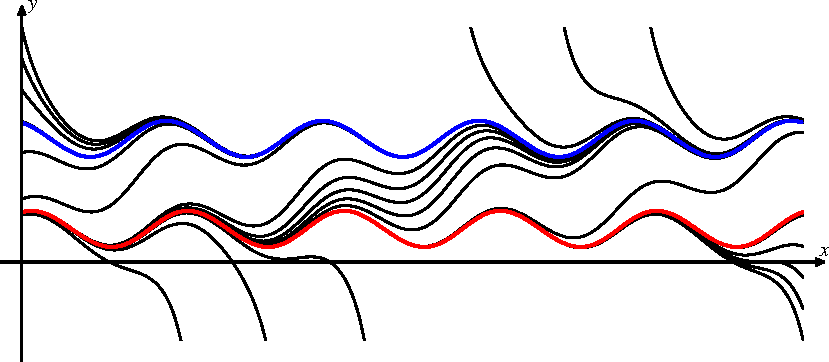
\includegraphics{chapters/images/geometrie-13.pdf}
\caption{Entwicklung des Systems~(\ref{geometrie:harvest-equation})
mit $a=5$ und $h=0.8$
\label{geometrie:harvest-graph}}
\end{figure}%
\end{refsection}

